\documentclass{report}
\usepackage[utf8]{inputenc}
\usepackage[T1]{fontenc}
\usepackage[swissgerman]{babel}
\usepackage[left=2cm,right=1.5cm,top=1.5cm,bottom=1.5cm]{geometry}
\usepackage{amssymb}
\usepackage{ragged2e}
\usepackage{titlesec}
\usepackage{booktabs}
\usepackage{svg}
\usepackage{transparent}
\usepackage{float}
\usepackage{hyperref}
\usepackage[many]{tcolorbox}
\usepackage{epigraph}
\usepackage{listings}

\lstloadlanguages{Java,Ruby}
\lstdefinestyle{fmo}{
  keywordstyle=\color{blue},
  identifierstyle=\bfseries\color{black},
  frame=single,
  basicstyle=\footnotesize\ttfamily,
  showstringspaces=false,
  keepspaces=true,
}
\lstset{style=fmo}

\setsvg{inkscape=inkscape -z -D,svgpath=__src/svg/}

\setlength\parindent{0pt}
\linespread{1.3}

\titleformat{\chapter}[display]
{\normalfont\huge\bfseries}{\chaptertitlename\ \thechapter}{20pt}{\Huge}
\titlespacing*{\chapter}{0pt}{0pt}{40pt}

%\renewcommand{\labelenumi}{\alph{enumi}.}

\newcommand{\pro}[1]{\item [pro]#1}
\newcommand{\con}[1]{\item [con]#1}

\newtcolorbox{caveat}[1][]{
  breakable,
  freelance,
  title=CAVEAT: #1,
  colback=white,
  colbacktitle=white,
  coltitle=black,
  fonttitle=\bfseries,
  bottomrule=0pt,
  boxrule=0pt,
  colframe=white,
  overlay unbroken and first={
    \draw[red!75!black,line width=3pt]
    ([xshift=5pt]frame.north west) -- 
    (frame.north west) -- 
    (frame.south west);
    \draw[red!75!black,line width=3pt]
    ([xshift=-5pt]frame.north east) -- 
    (frame.north east) -- 
    (frame.south east);
  },
  overlay unbroken app={
    \draw[red!75!black,line width=3pt,line cap=rect]
    (frame.south west) -- 
    ([xshift=5pt]frame.south west);
    \draw[red!75!black,line width=3pt,line cap=rect]
    (frame.south east) -- 
    ([xshift=-5pt]frame.south east);
  },
  overlay middle and last={
    \draw[red!75!black,line width=3pt]
    (frame.north west) -- 
    (frame.south west);
    \draw[red!75!black,line width=3pt]
    (frame.north east) -- 
    (frame.south east);
  },
  overlay last app={
    \draw[red!75!black,line width=3pt,line cap=rect]
    (frame.south west) --
    ([xshift=5pt]frame.south west);
    \draw[red!75!black,line width=3pt,line cap=rect]
    (frame.south east) --
    ([xshift=-5pt]frame.south east);
  },
}

\newtcolorbox{additional}[1][]{
  breakable,
  freelance,
  title=Additional Resources: #1,
  colback=white,
  colbacktitle=white,
  coltitle=black,
  fonttitle=\bfseries,
  bottomrule=0pt,
  boxrule=0pt,
  colframe=white,
  overlay unbroken and first={
    \draw[green!75!black,line width=3pt]
    ([xshift=5pt]frame.north west) -- 
    (frame.north west) -- 
    (frame.south west);
    \draw[green!75!black,line width=3pt]
    ([xshift=-5pt]frame.north east) -- 
    (frame.north east) -- 
    (frame.south east);
  },
  overlay unbroken app={
    \draw[green!75!black,line width=3pt,line cap=rect]
    (frame.south west) -- 
    ([xshift=5pt]frame.south west);
    \draw[green!75!black,line width=3pt,line cap=rect]
    (frame.south east) -- 
    ([xshift=-5pt]frame.south east);
  },
  overlay middle and last={
    \draw[green!75!black,line width=3pt]
    (frame.north west) -- 
    (frame.south west);
    \draw[green!75!black,line width=3pt]
    (frame.north east) -- 
    (frame.south east);
  },
  overlay last app={
    \draw[green!75!black,line width=3pt,line cap=rect]
    (frame.south west) --
    ([xshift=5pt]frame.south west);
    \draw[green!75!black,line width=3pt,line cap=rect]
    (frame.south east) --
    ([xshift=-5pt]frame.south east);
  },
}

\title{POSA 1 - HS2015}

\author{Valentin \textsc{Meier}\\\\Vorlage von Felix \textsc{Morgner}}

\date{\today}

\begin{document}

\maketitle
\clearpage
\vspace*{\fill}
  \epigraph{Sometimes the questions are complicated and the answers are simple.}{Dr. Seuss}
\vfill
\clearpage

\setcounter{tocdepth}{0}
\tableofcontents

\chapter{Layers}

\section{Summary}
Das Layer Pattern hilft Applikationen zu strukturieren, welche in Gruppen von Teilaufgaben zerteilt werden können so dass, jede Gruppe auf einem bestimmten Abstraktionslevel ist.
\section{Context}
Ein grosses System das Zerlegung benötigt.

\section{Problem}
Ein grosses System mit Low- und Highlevel Problemen hat zu wenig Struktur. Die Highlevel-Probleme bauen dabei auf den Lowlevel-Problemen auf. Es ist schwer Wartbar und die Aufgaben und Grenzen zwischen den Komponenten sind ungenau.

Ein mögliches Beispiel für ein solches System ist ein Netzwerk. Dabei ist ein Lowlevel-Problem: \textit{"Wie bringe ich Daten von A nach B?"} und ein Highlevel-Problem: \textit{"Wie ordne ich verschiedene Pakete einer logischen Session zu?"}

\section{Solution}
Das System wird in beliebig viele Layer aufgeteilt. Die Layer bauen aufeinander auf, wobei der höchste Layer den höchsten Abstraktionsgrad hat. Alle Komponenten mit dem selben Abstrationsgrad befinden sich auf dem selben Layer. Jedem Layer werden bestimmte Aufgaben zugewiesen. Er nutzt jeweils die Services des eins tieferen Layers. \\\\
Bei vielen Komponenten pro Layer wird je Layer ein Interface Objekt definiert welches mit den anderen Layern kommuniziert. Meist wird aus einem Request (Zugriff von Oben nach Unten) mehrere je tiefer der Request in den Layern nach unten wandert. Das Umgekehrte gilt bei einer Notification (Zugriff von Unten nach Oben).
Die folgenden Schritte beschreiben einen schrittweisen Ansatz zur Definition einer Layer Architektur. Dies ist nicht immer die beste Lösung. Es sind auch nicht alle Schritte zwingend notwendig. Vorgehen:
\begin{enumerate}
	\item Abstraktionskriterien definieren (Wie die Layer sich abgrenzen)
	\item Anzahl Abstraktionslevel definieren
	\item Layers benennen und Tasks zuteilen
	\item Services pro Layer spezifizieren
	\item 1.-4. zur Verfeinerung wiederholen
	\item Ein Interface pro Layer definieren, eventuell Facade Pattern anwenden
	\item Layer im Innern strukturieren (Bridge/Strategy Pattern)
	\item Kommunikation zwischen benachbarten Layern spezifizieren
	\item Benachbarte Layer entkuppeln (Bsp. One-Way Coupling/Retour mit Callbacks)
	\item Error Handling Strategie entwickeln. Entweder im Layer behandeln oder an den nächst höheren weitergeben. Faustregel:Am besten am tiefstmöglichen Layer behandeln.
\end{enumerate}
Es gibt noch zwei weitere Varianten des Layer Pattern:
\begin{description}
	\item[Relaxed Layered System] Layer können Services aller unterliegenden Layer benutzen. Mehr Flexibilität und Performance, jedoch schlechtere Wartbarkeit.
	\item[Layering through inheritance] Für OO-Systeme. Lower Layer als base classes. Höhere Layer erben von diesen. So können höhere Layer Funktionalität von tieferen ihren Bedürfnissen anpassen.
\end{description}

\subsection{Structure}

\begin{figure}[H]
  \centering
  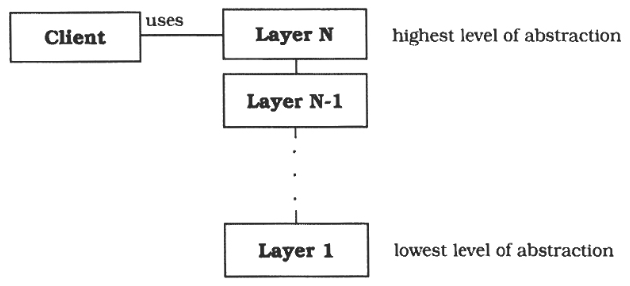
\includegraphics[width=0.8\textwidth]{figures/00-layers-1}
  \caption{Illustration des Layer-Patterns}
\end{figure}

\section{Consequences}
\begin{itemize}
    \pro{Wiederverwendbarkeit von Layern}
    \pro{Austauschbarkeit von Layern}
    \pro{Support für Standardisierung}
    \pro{Dependencies bleiben lokal}
    \con{Tiefere Effizienz}
    \con{Mehr Aufwand}
    \con{Schwierigkeit beim bestimmen der Granularität der Layer}
    \con{Jeder Layer-Übergang schmälert die Performance}
\end{itemize}

\section{Known Uses}
\begin{itemize}
	\item OSI Protocol Stack 
	\item Virtual Machines
	\item APIs
	\item Information Systems
	\item Windows NT
\end{itemize}

\section{Relationships}
\begin{itemize}
	\item \textit{Composite Message} beschreibt eine objekt-orientierte Verschachtelung von Nachrichten, welche durch die Schichten transportiert werden. Eine Composite Message ist ein Paket, welches aus header, payload und eingebetteten Paketen besteht.
	\item \textit{Mikrokernel Architecture} kann als spezialisierte Layer-Architektur angesehen werden.
\end{itemize}

\section{Exam Questions}
\begin{itemize}
  \item Behauptung: Etwas zu bottom-up dekouplung in layer? (Lösung)
    \item Frage: Welches GOF Pattern hilft bei der definierung von Interfaces im Layers Pattern? (Facace Pattern)
\end{itemize}


\clearpage
\vspace*{\fill}
\begin{center}
    { \huge \bfseries :wq }
\end{center}
\vfill
\clearpage


\end{document}
